\documentclass[11pt,a4paper,UTF8,fontset=windows]{ctexart}

\usepackage[margin=2.35cm,top=2.5cm,bottom=2.4cm]{geometry}
\usepackage{amsmath,amssymb,bm}
\usepackage{booktabs,tabularx,multirow,array}
\usepackage{graphicx}
\usepackage{float}
\usepackage{enumitem}
\usepackage{xcolor}
\usepackage{pgfplots}
\pgfplotsset{compat=1.18}
\usepgfplotslibrary{groupplots}
\usepackage{tikz}
\usetikzlibrary{positioning,arrows.meta,calc,fit,backgrounds}
\usepackage{needspace}
\usepackage[hidelinks]{hyperref}
\usepackage{caption}
\captionsetup{font=small,labelfont=bf,skip=4pt}

\definecolor{navy}{HTML}{234E70}
\definecolor{teal}{HTML}{2A9D8F}
\definecolor{coral}{HTML}{E76F51}
\definecolor{rose}{HTML}{C94C6D}
\definecolor{gold}{HTML}{D9A441}
\definecolor{sage}{HTML}{7A9E7E}
\definecolor{mist}{HTML}{F4F6F8}

\setlength{\parskip}{0pt}
\setlength{\parindent}{2em}
\setlength{\emergencystretch}{2.5em}
\linespread{1.18}
\setlength{\tabcolsep}{5pt}
\renewcommand{\arraystretch}{1.16}

\ctexset{
  section/format = \Large\bfseries,
  subsection/format = \large\bfseries,
  subsubsection/format = \normalsize\bfseries,
}

\newcommand{\best}[1]{\textbf{#1}}
\newcommand{\pp}{\,\text{pp}}

\begin{document}
\pagestyle{plain}

\begin{center}
{\LARGE\bfseries 花间识微：面向小规模五类花卉细粒度分类的\\[2pt]
数据审计与迁移集成框架\par}
\vspace{0.6em}
{\normalsize Reading Petals: A Data-Auditing and Transfer-Ensemble Framework for\\[2pt]
Fine-Grained Five-Class Flower Classification with Small Data\par}
\end{center}

\vspace{0.6em}

\begin{abstract}
花卉识别是典型的细粒度视觉任务：类间差异常小于类内差异，公开数据中又混有无关图像。本文提出一套面向小规模、标签带噪花卉数据的数据审计与迁移集成框架。框架由三部分组成：以 MD5/dHash 聚类为单位的去泄漏划分、置信度排序—物体筛查—原图与来源复核的三级标签审计，以及从零结构到 ImageNet 预训练主干的受控训练与概率集成。在 3{,}670 张五类图像上，框架将评测口径与模型选择分开：从零训练的最佳结构 ResidualCNN+SE（1.23M 参数）达到 86.39\% 测试准确率；迁移学习将单模型提升至 96.91\%，256 输入降低 roses/tulips 的验证集双向混淆（16$\rightarrow$10）；ConvNeXt-Base-256 与 EfficientNetV2-M-224 的等权概率集成在清洗测试集（$n=544$）上取得 \best{97.43\%} 准确率与 \best{0.9737} Macro-F1，错误 14 个。清洗使评测口径更可靠，但清洗后重训（96.69\%）低于原模型（96.88\%），表明限制性能的主要因素已由标签噪声转向任务可分性与样本规模。二项标准误约 0.7\pp；97.4\% 只适用于当前标注版本与测试集。

\par\medskip
\noindent\textbf{关键词：} 细粒度图像分类；卷积神经网络；迁移学习；通道注意力；集成学习；标签噪声；可复现性
\end{abstract}

\vspace{0.4em}
{\small
\noindent\textbf{Abstract.}\quad Flower recognition is a fine-grained vision problem: between-class differences can be smaller than within-class variation, and community datasets often contain irrelevant images. This paper presents a data-auditing and transfer-ensemble framework for small, label-noisy flower datasets. The framework has three components: cluster-level splitting based on MD5/dHash to prevent near-duplicate leakage, a three-stage label audit (confidence ranking, object screening, and source verification), and controlled training with probability ensembling from scratch CNNs to ImageNet-pretrained backbones. On 3{,}670 images from five classes, the framework separates evaluation conditions from model selection. The best from-scratch model (ResidualCNN+SE, 1.23M parameters) reaches 86.39\% test accuracy. Transfer learning raises a single model to 96.91\%, and 256-pixel inputs reduce roses/tulips confusion on validation from 16 to 10. An equal-weight ensemble of ConvNeXt-Base-256 and EfficientNetV2-M-224 attains 97.43\% accuracy and 0.9737 macro-F1 on the cleaned test set ($n=544$), with 14 errors. Cleaning improves evaluation hygiene but not accuracy upon retraining (96.69\% versus 96.88\%), indicating that the main limitation has shifted from label noise to task separability and sample size. The binomial standard error is about 0.7\pp; the 97.4\% result applies to the current annotation version and test set.

\medskip
\noindent\textbf{Keywords:} fine-grained image classification; convolutional neural networks; transfer learning; channel attention; ensemble learning; label noise; reproducibility\par}

\vspace{0.6em}

\section{引言}

\subsection{问题背景}

花卉识别属于细粒度视觉分类：类别由花瓣形状、层次、花心结构和色彩共同决定，类间差异可能小于同一种花卉在花苞、盛放、凋谢、特写与远景下的外观差异。公开图像多来自 Flickr，拍摄距离、光照、背景和后期风格不受控，模型容易把草地、花园栅栏或暖色调当作类别线索。本文使用的五类花卉数据只有约 2.5k 张训练图，从零训练难以获得稳定的细粒度表征。其中 roses 与 tulips 的花型、花瓣层次接近，是本文最难的混淆对。

这些因素使分类性能同时受模型、数据和评测口径影响。只比较网络结构，无法判断增益来自容量、预训练还是标签质量；只在含噪测试集上报告准确率，也无法区分模型误差与标注错误。模型设计的目标是：在不增加标注成本的前提下，利用 ImageNet 预训练表征降低 roses/tulips 的混淆，并用互补分支减少单模型的偶然错误。

\subsection{主要贡献}

本文的贡献有三点。第一，提出以 MD5/dHash 聚类为单位的去泄漏划分与三级标签审计流程，形成逐条可追溯的清洗版数据。第二，在同一协议下构建受控训练与评估流程，覆盖 5 种从零结构、4 种增强策略、3 个预训练主干、2 种输入分辨率以及 TTA 与概率集成。第三，在 3{,}670 张五类图像上验证该框架，并给出二项标准误与选择偏差分析。

\subsection{与已有工作的关系}

细粒度识别的主流路线有三类：一是部件/双线性表示，通过定位判别性部位或建模二阶特征提升类间可分性\cite{lin2015bilinear,wei2022fgia}；二是强主干与迁移学习，自 AlexNet\cite{krizhevsky2012alexnet} 以来，卷积网络在大规模数据上预训练学习通用视觉表征，再在小数据集上微调\cite{he2016resnet,liu2022convnext,tan2021effnetv2}；三是数据与训练策略，包括数据增强、标签平滑、EMA、TTA 与集成\cite{zhang2018mixup,szegedy2016inception,tarvainen2017mean,dietterich2000ensemble}。本文将这些手段组织为一个面向小规模、标签带噪数据的框架，并在同一评测口径下验证其收益与边界。

在数据侧，Nilsback 与 Zisserman 的工作表明，花卉数据集的类别边界与拍摄条件会显著影响识别难度\cite{nilsback2008flower}；在标签侧，Confident Learning 一类方法强调应显式估计“标注是否可信”，而不是把测试集当作金标准\cite{northcutt2021confident}。本文的标签审计受这一思想影响，但保留人工最终裁决，避免用模型预测替代事实判断。

\section{模型设计}

\subsection{最终方案}

最终方案由两个互补的卷积分支组成：同一张花卉图像分别经过 ConvNeXt-Base-256 与 EfficientNetV2-M-224，得到两组五类概率，再等权平均。图~\ref{fig:architecture} 给出推理流程。分支 A 使用 $256\times256$ 输入（短边缩放 288 后中心裁剪），分支 B 使用 $224\times224$ 输入（短边缩放 256 后中心裁剪）。两个分支都从 ImageNet 预训练权重初始化，替换 5 类分类头后全参数微调。

推理时，每个分支先对原图与水平翻转图分别前向，平均两次 softmax 输出；两个分支的概率再等权平均，取最大概率类别：
\begin{equation}
\bar p(y\mid x)=\frac{1}{4}\sum_{m\in\{A,B\}}\sum_{t\in\{0,1\}}p_m\!\left(y\mid T_t(x)\right),
\qquad
\hat y=\arg\max_y \bar p(y\mid x),
\label{eq:final-ensemble}
\end{equation}
其中 $T_0$ 为恒等变换，$T_1$ 为水平翻转。两个分支的参数量分别为 87.57M 与 52.86M，合计约 140M；推理需要 4 次前向（两模型 $\times$ 翻转 TTA）。

\begin{figure}[htbp]
\centering
\begin{tikzpicture}[scale=0.88, transform shape, font=\scriptsize,
  box/.style={draw=navy!55, fill=navy!4, rounded corners=1.5pt, align=center, inner sep=3pt, minimum height=9mm, text width=2.4cm},
  branch/.style={box, fill=teal!7, draw=teal!60},
  merge/.style={box, fill=gold!10, draw=gold!70},
  finalbox/.style={box, fill=coral!8, draw=coral!65},
  arr/.style={-{Stealth[length=1.6mm]}, draw=navy!60, line width=0.6pt}
]
\node[draw=navy!55, fill=white, rounded corners=1.5pt, inner sep=2pt, align=center] (input) at (0,0) {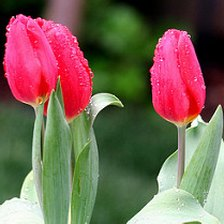
\includegraphics[width=1.5cm]{figures/architecture_input.jpg}\\[1pt]\scriptsize 输入图像};
\node[branch] (preA) at (3.2,1.55) {短边缩放 288\\中心裁剪 $256\times256$};
\node[branch] (cnnA) at (6.3,1.55) {ConvNeXt-Base\\ImageNet 预训练\\87.57M};
\node[branch] (probA) at (9.6,1.55) {5 类 softmax $p_A$\\翻转 TTA 平均};
\node[branch] (preB) at (3.2,-1.55) {短边缩放 256\\中心裁剪 $224\times224$};
\node[branch] (cnnB) at (6.3,-1.55) {EfficientNetV2-M\\ImageNet 预训练\\52.86M};
\node[branch] (probB) at (9.6,-1.55) {5 类 softmax $p_B$\\翻转 TTA 平均};
\node[merge] (avg) at (12.8,0) {等权平均\\$\bar p=(p_A+p_B)/2$};
\node[finalbox, text width=2.0cm] (arg) at (15.3,0) {$\arg\max$\\最终类别};
\draw[arr] (input.east) -- ++(0.45,0) |- (preA.west);
\draw[arr] (input.east) -- ++(0.45,0) |- (preB.west);
\draw[arr] (preA) -- (cnnA);
\draw[arr] (cnnA) -- (probA);
\draw[arr] (preB) -- (cnnB);
\draw[arr] (cnnB) -- (probB);
\draw[arr] (probA.east) -- ++(0.4,0) |- (avg.west);
\draw[arr] (probB.east) -- ++(0.4,0) |- (avg.west);
\draw[arr] (avg) -- (arg);
\node[font=\scriptsize\bfseries, text=teal!80!black, above=4mm of cnnA] {分支 A：EMA 0.995};
\node[font=\scriptsize\bfseries, text=teal!80!black, below=4mm of cnnB] {分支 B：无 EMA};
\begin{scope}[on background layer]
\node[draw=teal!40, dashed, rounded corners=3pt, fit=(preA)(probA), inner sep=4pt] {};
\node[draw=teal!40, dashed, rounded corners=3pt, fit=(preB)(probB), inner sep=4pt] {};
\end{scope}
\end{tikzpicture}
\caption{最终方案。两个分支分别输出五类概率，经翻转 TTA 与等权平均后取最大概率类别。}
\label{fig:architecture}
\end{figure}

\subsection{分支训练}

ConvNeXt-Base 分支使用 $256\times256$ 输入，训练 6 个 epoch，AdamW（$lr=2\times10^{-5}$，$wd=0.01$），余弦退火，标签平滑 0.1，EMA 衰减 0.995，batch size 32。EfficientNetV2-M 分支使用 $224\times224$ 输入，训练 5 个 epoch，AdamW（$lr=10^{-4}$，$wd=10^{-4}$），标签平滑 0.1，不使用 EMA。训练目标为标签平滑交叉熵（$\varepsilon=0.1$）；两个分支都使用随机缩放裁剪、水平翻转与颜色抖动，验证与测试只做确定性缩放和中心裁剪。

选择这两个分支的依据是归纳偏置的互补性。ConvNeXt 的 $7\times7$ 深度可分离卷积与大核设计偏向形状与全局结构；EfficientNetV2-M 的复合缩放与 MBConv/Fused-MBConv 偏向多尺度纹理。二者在不同分辨率下训练，错误相关性较低。EMA 只用于 ConvNeXt 分支：该分支训练轮数略多，滑动平均能降低模型选择的方差；EfficientNet 分支在 5 轮内已收敛，EMA 的收益有限。

\subsection{对照模型}

为判断最终方案的收益，本文保留三类对照。SimpleCNN 由 4 个卷积块组成，通道数 $32\to64\to128\to256$，全局平均池化后接 5 类线性层，约 1.17M 参数。ResidualCNN 在相同通道计划上加入残差捷径，通道变化时用 $1\times1$ 卷积投影，约 1.22M 参数；Residual+SE 在后两个 stage 加入压缩比 16 的 SE 通道注意力，约 1.23M 参数。迁移对照包括 MobileNetV3-Small（1.52M 参数）与 EfficientNetV2-M（52.86M 参数），训练配置与分支 B 相同或更短。所有对照使用同一划分、同一评估变换与同一随机种子。

\section{数据与实验设置}

\subsection{数据概况}

数据集包含 5 个类别、3{,}670 张 JPEG 图像，全部为 RGB，无损坏文件。表~\ref{tab:stats} 汇总了类别规模与基本视觉统计。dandelion 最多（898 张，24.5\%），daisy 最少（633 张，17.2\%），最大/最小类别比约 1.42，属于轻度不平衡；因此本文只使用分层划分，不做重采样或类别加权，以免把“类别先验”与“模型能力”混在一起。

\begin{table}[htbp]
\centering
\small
\caption{数据集类别分布与视觉统计。短边$\geq$224 表示该比例的原图在 224 输入下不需要上采样。亮度与饱和度归一化到 $[0,1]$。}
\label{tab:stats}
\begin{tabular}{lrrrrrrr}
\toprule
类别 & 图像数 & 占比 & 平均尺寸 & 宽高比 & 短边$\geq$224 & 亮度 & 饱和度 \\
\midrule
daisy      & 633 & 17.2\% & $359\times271$ & 1.31 & 72.5\% & 0.48 & 0.42 \\
dandelion  & 898 & 24.5\% & $367\times274$ & 1.32 & 77.5\% & 0.47 & 0.48 \\
roses      & 641 & 17.5\% & $364\times275$ & 1.31 & 79.1\% & 0.53 & 0.47 \\
sunflowers & 699 & 19.0\% & $360\times270$ & 1.32 & 73.4\% & 0.56 & 0.59 \\
tulips     & 799 & 21.8\% & $372\times269$ & 1.37 & 65.0\% & 0.54 & 0.51 \\
\midrule
合计       & 3{,}670 & 100\% & $365\times272$ & 1.33 & 73.4\% & 0.52 & 0.49 \\
\bottomrule
\end{tabular}
\end{table}

图~\ref{fig:data-overview} 的两个统计直接影响输入设计。左图显示分层划分后的类别比例与原始分布一致；右图给出短边累积分布：73.4\% 的图像短边不小于 224，35.0\% 不小于 288。把输入从 224 提到 256（短边缩放 288）时，约 65\% 的样本仍要上采样，原生细节有限。这一约束解释了后文 256 输入只在 roses/tulips 等难类上带来小幅改善，而不改变总体测试准确率。


\begin{figure}[H]
\centering
\begin{tikzpicture}
\begin{groupplot}[
  group style={group size=2 by 1, horizontal sep=1.1cm},
  width=0.47\linewidth, height=5.4cm,
  axis lines=left, tick label style={font=\scriptsize},
  label style={font=\small}, title style={font=\small\bfseries},
  ymajorgrids, grid style={gray!15},
]
\nextgroupplot[
  ybar stacked, bar width=9pt,
  symbolic x coords={daisy,dandelion,roses,sunflowers,tulips},
  xtick=data, xticklabel style={font=\scriptsize,rotate=18,anchor=north east},
  ymin=0, ymax=950, ylabel={图像数}, title={(a) 类别与划分},
  legend style={at={(0.5,-0.45)},anchor=north,legend columns=3,draw=none,font=\scriptsize},
  enlarge x limits=0.13,
]
\addplot[fill=navy!75,draw=navy] coordinates {
  (daisy,443) (dandelion,628) (roses,448) (sunflowers,487) (tulips,558)};
\addplot[fill=teal!65,draw=teal] coordinates {
  (daisy,95) (dandelion,135) (roses,96) (sunflowers,105) (tulips,120)};
\addplot[fill=gold!70,draw=gold] coordinates {
  (daisy,95) (dandelion,135) (roses,96) (sunflowers,105) (tulips,120)};
\legend{训练, 验证, 测试}
\nextgroupplot[
  xmin=120, xmax=470, ymin=0, ymax=104,
  xlabel={图像短边（像素）}, ylabel={短边$\geq x$ 的比例 (\%)},
  title={(b) 分辨率累积分布},
]
\addplot[color=teal, line width=1.1pt] table[x=threshold,y=cum_pct]
  {figures/short_side_cumulative.dat};
\addplot[gray, dashed, line width=0.6pt] coordinates {(224,0) (224,104)};
\addplot[gray, dashed, line width=0.6pt] coordinates {(288,0) (288,104)};
\node[font=\scriptsize,anchor=south west,text=gray!70] at (axis cs:226,8) {224};
\node[font=\scriptsize,anchor=south west,text=gray!70] at (axis cs:290,8) {288};
\end{groupplot}
\end{tikzpicture}
\caption{数据总览。(a) 分层划分后的类别构成；(b) 图像短边的累积分布，虚线标出 224 与 288 两个关键阈值。仅约 35\% 的图像能原生支持 288 短边，这限制了 256 输入的实际收益。}
\label{fig:data-overview}
\end{figure}

\subsection{颜色与背景偏置}

各类平均亮度在 0.47--0.56 之间，差异有限；色相分布差异明显：dandelion 与 sunflowers 集中在黄橙色相，roses 偏红/品红，daisy 与 tulips 更分散。仅用颜色直方图的线性分类器就能取得较高准确率，卷积网络也可能把背景颜色、草地比例和拍摄风格当作线索。类平均图显示各类构图与背景占比存在系统差异。为降低捷径风险，训练使用颜色抖动与随机缩放裁剪，并把增强消融作为独立实验检验颜色扰动的作用；Grad-CAM 定位分析留作后续工作。

\subsection{重复检测与数据划分}

重复样本是小型数据集上最常见的隐性泄漏源：同一张图或同一场景的轻微变体若同时出现在训练集与测试集，指标会被系统性高估。本文用两级指纹处理该问题。完全重复用文件 MD5 判定；近重复用 64 位 dHash：将图像转为 $9\times8$ 灰度图，比较水平相邻像素得到 64 位指纹 $h$，两张图像的汉明距离为
\begin{equation}
d_H(h_i,h_j)=\operatorname{popcount}(h_i\oplus h_j).
\label{eq:dhash}
\end{equation}
当 $d_H\le 4$ 时用并查集合并为同一簇，划分时以簇为最小单位，保证同一簇只进入训练/验证/测试集之一。

原始数据中检出 3 组完全重复（6 张）与 17 对近重复（34 张，占 0.9\%），其中 1 组完全重复跨类别冲突（同一张图同时出现在 roses 与 tulips，无法确定唯一标签）。处理策略是：跨类冲突整组剔除（2 张），同类完全重复每组保留一张（剔除 2 张），近重复簇整体分入同一划分。最终使用 3{,}666 张，按类别分层划分为 2{,}564 / 551 / 551（约 70\% / 15\% / 15\%），校验结果为 \best{0 个簇跨越划分}。表~\ref{tab:splits} 列出原始与清洗两个版本的逐类划分。

\begin{table}[htbp]
\centering
\small
\caption{两个数据版本的划分。原始版本用于训练与消融；清洗版用于最终评测。清洗只删除样本，不改变 划分归属，因此两版可逐样本对应。}
\label{tab:splits}
\begin{tabular}{lrrrrrrrr}
\toprule
\multirow{2}{*}{类别} & \multicolumn{3}{c}{原始划分（3{,}666）} & \multicolumn{4}{c}{清洗版（3{,}609）} & \multirow{2}{*}{剔除} \\
\cmidrule(lr){2-4}\cmidrule(lr){5-8}
 & 训练 & 验证 & 测试 & 训练 & 验证 & 测试 & 合计 & \\
\midrule
daisy      & 443 & 95  & 95  & 442 & 95  & 95  & 632 & 1 \\
dandelion  & 628 & 135 & 135 & 628 & 135 & 135 & 898 & 0 \\
roses      & 448 & 96  & 96  & 427 & 89  & 95  & 611 & 29 \\
sunflowers & 487 & 105 & 105 & 485 & 105 & 104 & 694 & 3 \\
tulips     & 558 & 120 & 120 & 545 & 114 & 115 & 774 & 24 \\
\midrule
合计       & 2{,}564 & 551 & 551 & 2{,}527 & 538 & 544 & 3{,}609 & 57 \\
\bottomrule
\end{tabular}
\end{table}

\subsection{预处理与增强}

所有图像统一转为 RGB，并按 ImageNet 统计量归一化：
\begin{equation}
\hat{x}_{c}=\frac{x_{c}-\mu_{c}}{\sigma_{c}},\qquad
\mu=(0.485,0.456,0.406),\quad
\sigma=(0.229,0.224,0.225).
\label{eq:normalize}
\end{equation}
224 模型采用 $\text{Resize}(256)\rightarrow\text{CenterCrop}(224)$；256 模型采用 $\text{Resize}(288)\rightarrow\text{CenterCrop}(256)$。训练增强包括随机缩放裁剪（面积比例 0.65--1.0，宽高比 0.8--1.25）、水平翻转与颜色抖动（亮度/对比度/饱和度 0.2，色相 0.05）；关于图像增强的系统综述可参见\cite{shorten2019augmentation}。验证与测试只做确定性的缩放与中心裁剪，且同一张图两次前向的输出完全一致。图~\ref{fig:preprocess} 显示同一张图在四种变换下的视图；随机裁剪会改变构图与背景比例，这类与类别无关的因素应尽量从模型中排除。

\begin{figure}[htbp]
\centering
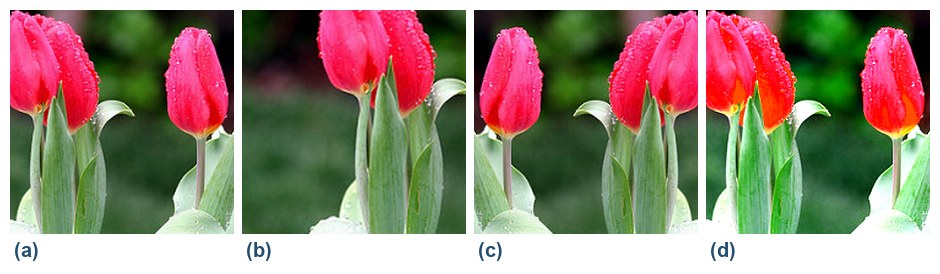
\includegraphics[width=0.95\linewidth]{figures/preprocess_examples.jpg}
\caption{预处理与增强示例。(a) 确定性中心裁剪（验证/测试）；(b) 随机缩放裁剪；(c) 水平翻转；(d) 颜色抖动（近似训练时的 ColorJitter）。(b)--(d) 只作用于训练集。}
\label{fig:preprocess}
\end{figure}



\subsection{标签审计与两版测试集}

\subsubsection{动机}

误差分析中有一类错误无法由模型能力解释：roses 的错分样本中有车辆、建筑和食物，tulips 的错分样本中有风信子田。若测试集包含这类图像，准确率同时低估模型能力并高估数据质量；训练集中的无关图像还会把非花卉概念带入决策边界。标签审计因此与模型训练同等重要。审计要回答的是一个可核查的问题：这张图是否确实包含该类别定义下的真实花卉？只有确定不包含或确定属于另一物种时才删除；对“有花但物种存疑”的样本保守保留。

\subsubsection{审计流程}

审计分三步：用训练好的 ConvNeXt-Base 对全部图像推理，按最大 softmax 置信度升序排列，并导出验证集与测试集的错分样本；用 ImageNet 预训练分类器筛查车辆、建筑、动物、景观、食物和人物活动等非花卉候选；对争议样本查看高分辨率原图，结合 Flickr 页面标题、作者标签与 oEmbed 元数据确认拍摄对象，无法确认时保留并记录复核标记。最终清单包含 64 条决策：57 条排除、7 条保留；每条记录保留证据与来源，便于追溯。

\subsubsection{判定准则}

排除的对象是图中不存在符合类别定义的真实花卉，或内容为车辆、建筑、风景、人物活动、食物、插画/装饰等明确无关对象，或主体明显属于另一物种（如把风信子标成 tulips）。图中存在目标花卉但物种或品种存疑、混合场景中目标可见、或为可识别的营养器官与种子头时，保留样本并记录不确定性。清洗只做删除，保持原划分归属；两版共享同一评估协议，清洗前后的差异可归因于样本集合变化，而不是划分变化。

\subsubsection{审计结果}

审计共排除 57 张（训练集 37、验证集 13、测试集 7），占 3{,}666 张的 1.55\%。按问题类型可分为三类（表~\ref{tab:audit}、图~\ref{fig:audit}）：\textbf{无关场景或物体} 31 张（车辆、建筑、人物活动、食物、喷泉、茶杯等），\textbf{非真实花卉描绘} 19 张（绘画、插画、装饰、蛋糕糖霜花、光雕），\textbf{类别不符} 7 张（风信子田、非玫瑰的复合花、三叶草、蓝色穗状花境等）。图~\ref{fig:noise} 展示 6 个例子，覆盖上述三类。

\begin{table}[htbp]
\centering
\small
\caption{清洗版的排除清单统计。占比以 57 张排除样本为分母。}
\label{tab:audit}
\begin{tabular}{lrrrrr}
\toprule
问题类型 & 训练 & 验证 & 测试 & 合计 & 占排除数 \\
\midrule
无关场景或物体 & 24 & 4 & 3 & 31 & 54.4\% \\
非真实花卉描绘 & 9  & 7 & 3 & 19 & 33.3\% \\
类别不符（另一物种） & 4 & 2 & 1 & 7 & 12.3\% \\
\midrule
合计 & 37 & 13 & 7 & 57 & 100\% \\
\bottomrule
\end{tabular}
\end{table}

\begin{figure}[htbp]
\centering
\begin{tikzpicture}
\begin{axis}[
  width=0.86\linewidth, height=5.2cm,
  xbar stacked, bar width=9pt,
  xmin=0, xmax=36,
  symbolic y coords={mismatch,nonphoto,scene},
  ytick=data,
  yticklabels={类别不符 (7), 非真实描绘 (19), 无关场景/物体 (31)},
  yticklabel style={font=\small},
  xlabel={图像数}, xlabel style={font=\small},
  tick label style={font=\scriptsize},
  legend style={at={(0.5,1.03)},anchor=south,legend columns=3,draw=none,font=\scriptsize},
  axis lines=left, xmajorgrids, grid style={gray!15},
  enlarge y limits=0.18,
]
\addplot[fill=navy!75,draw=navy] table[x=train,y=category] {figures/label_audit.dat};
\addplot[fill=teal!65,draw=teal] table[x=val,y=category] {figures/label_audit.dat};
\addplot[fill=gold!70,draw=gold] table[x=test,y=category] {figures/label_audit.dat};
\legend{训练, 验证, 测试}
\end{axis}
\end{tikzpicture}
\caption{标签审计的排除构成。大多数被排除样本位于训练集，但测试集的 7 张排除会直接改变最终评测口径（551$\rightarrow$544）。}
\label{fig:audit}
\end{figure}

\begin{figure}[htbp]
\centering
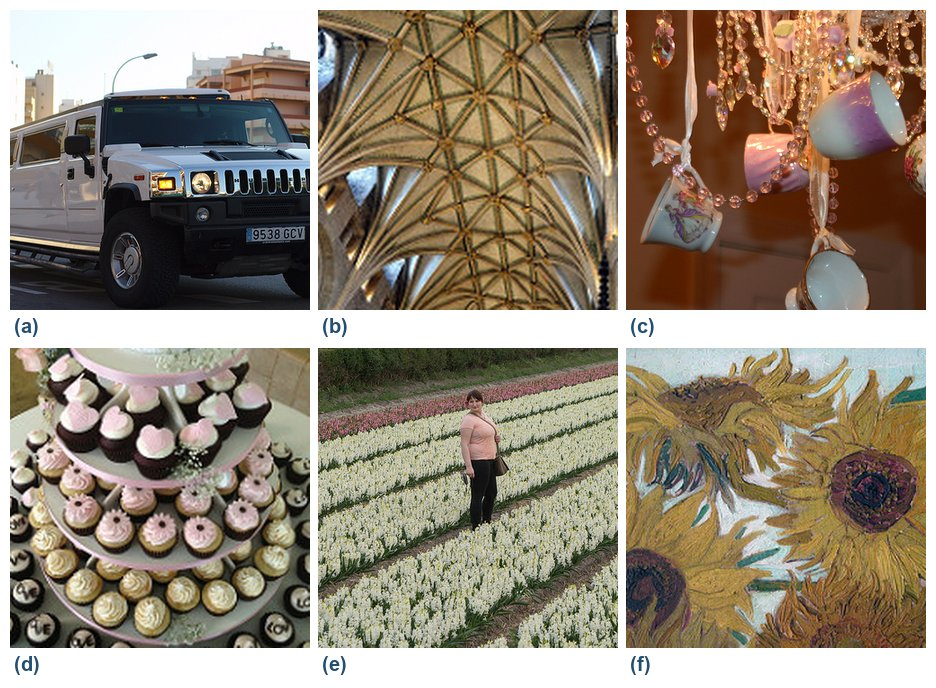
\includegraphics[width=0.9\linewidth]{figures/label_noise_examples.jpg}
\caption{标签噪声示例（均为原图中心裁剪）。(a) 白色悍马车被标为 roses；(b) 哥特式穹顶被标为 roses；(c) 茶杯挂饰被标为 roses；(d) 纸杯蛋糕塔被标为 roses；(e) 风信子花田被标为 tulips；(f) 向日葵油画被标为 sunflowers。}
\label{fig:noise}
\end{figure}

\subsubsection{审计的边界}

审计是候选驱动的：复核范围是 383 张高风险候选，57 张是已确认无关的数量，数据集的真实噪声率可能更高。测试集删除 7 张（551$\rightarrow$544），roses 与 tulips 分别减少 1 张和 5 张，逐类指标约有 0.5--1\pp 的波动，比较必须在同一测试集上进行。清洗只移除错误监督，不增加新信息，不能保证重训一定更好；第~\ref{sec:results} 节的结果说明了这一点。


\subsection{数据与评估流程}

该框架需要同时处理两个问题：训练与评测之间的近重复泄漏，以及模型误差与标签误差的区分。图~\ref{fig:pipeline} 概括了处理流程。原始图像先按 MD5 与 dHash 聚类，去重后以簇为单位分层划分为 2{,}564 / 551 / 551；随后用训练好的 ConvNeXt 排序候选、用 ImageNet 分类器筛查非花卉物体，再结合原图与 Flickr 元数据人工复核，得到 2{,}527 / 538 / 544 的清洗版划分。原始划分用于训练与早期消融，清洗版只用于最终评测；清洗只删除样本、不改变样本归属，因此两版指标可以逐样本对应。

\begin{figure}[htbp]
\centering
\begin{tikzpicture}[font=\scriptsize]
\tikzset{
  stage/.style={draw, rounded corners=2pt, minimum height=11mm,
    text width=150mm, align=left, inner sep=4pt},
  arr/.style={-{Stealth[length=1.7mm]}, draw=navy!55, line width=0.7pt}
}
\node[stage, fill=teal!5, draw=teal!55] (s1) at (0,0)
  {\textbf{\color{teal}1.\ 数据}\quad
   \colorbox{teal!12}{原始 3{,}670}\ \ $\rightarrow$\ \
   \colorbox{teal!12}{MD5 + dHash 去重 3{,}666}\ \ $\rightarrow$\ \
   \colorbox{teal!12}{簇级分层 2{,}564 / 551 / 551}};
\node[stage, fill=gold!6, draw=gold!60] (s2) at (0,-16mm)
  {\textbf{\color{gold!80!black}2.\ 标签审计}\quad
   \colorbox{gold!14}{模型置信度排序}\ \ $\rightarrow$\ \
   \colorbox{gold!14}{ImageNet 物体筛查}\ \ $\rightarrow$\ \
   \colorbox{gold!14}{原图 + Flickr 来源复核}\ \ $\rightarrow$\ \
   \colorbox{gold!14}{清洗版 2{,}527 / 538 / 544}};
\node[stage, fill=coral!5, draw=coral!55] (s3) at (0,-32mm)
  {\textbf{\color{coral}3.\ 建模}\quad
   \colorbox{coral!12}{从零 CNN：Simple / Residual / +SE（5 组）}\ \ $\bullet$\ \
   \colorbox{coral!12}{迁移：MobileNetV3-S / EfficientNetV2-M / ConvNeXt-B}\ \ $\bullet$\ \
   \colorbox{coral!12}{输入 224 / 256}};
\node[stage, fill=navy!4, draw=navy!50] (s4) at (0,-48mm)
  {\textbf{\color{navy}4.\ 训练与推理}\quad
   \colorbox{navy!8}{AdamW + 余弦退火}\ \ $\bullet$\ \
   \colorbox{navy!8}{标签平滑 0.1}\ \ $\bullet$\ \
   \colorbox{navy!8}{EMA 0.995}\ \ $\bullet$\ \
   \colorbox{navy!8}{水平翻转 TTA}\ \ $\bullet$\ \
   \colorbox{navy!8}{等权概率集成}};
\node[stage, fill=sage!7, draw=sage!60] (s5) at (0,-64mm)
  {\textbf{\color{sage!70!black}5.\ 评测}\quad
   \colorbox{sage!14}{验证集选型}\ \ $\rightarrow$\ \
   \colorbox{sage!14}{测试集 Acc / Macro-F1}\ \ $\rightarrow$\ \
   \colorbox{sage!14}{混淆矩阵与逐样本误差}\ \ $\rightarrow$\ \
   \colorbox{sage!14}{标签边界复核}};
\foreach \a/\b in {s1/s2, s2/s3, s3/s4, s4/s5}
  \draw[arr] (\a.south) -- (\b.north);
\end{tikzpicture}
\caption{研究框架。数据侧先做去重与簇级分层，再做标签审计；模型侧在同一划分上完成从零训练、迁移学习与集成；最终在 清洗版测试集上报告结果，并把残余错误反馈到标签边界复核。}
\label{fig:pipeline}
\end{figure}


\subsection{训练与评估协议}

\subsubsection{实验环境与统一协议}

全部实验在单张 NVIDIA GeForce RTX 5090 Laptop GPU（24{,}463 MiB）上完成，Python 3.12 + PyTorch 2.x（CUDA 13.0），混合精度训练。所有模型共享同一份划分清单、同一套评估变换与同一随机种子（42），主要配置见表~\ref{tab:setup}。

\begin{table}[htbp]
\centering
\footnotesize
\caption{实验矩阵。所有模型均使用 AdamW、余弦退火与标签平滑 0.1；迁移模型另加 EMA 与 TTA。}
\label{tab:setup}
\begin{tabular}{llrrrll}
\toprule
阶段 & 模型 & 输入 & epochs & 学习率 & 正则 & 目的 \\
\midrule
基线 & SimpleCNN & 224 & 30 & $10^{-3}$ & -- & 建立参照 \\
长训练 & SimpleCNN & 224 & 80 & $10^{-3}$ & -- & 训练长度效应 \\
结构 & Residual / deep / +SE & 224 & 80 & $10^{-3}$ & -- & 归纳偏置 \\
增强 & 旋转 / 裁剪 / hue / Mixup & 224 & 80 & $10^{-3}$ & -- & 增强策略 \\
迁移 & MobileNetV3-Small & 224 & 8 & $3\times10^{-4}$ & -- & 轻量部署 \\
迁移 & EfficientNetV2-M & 224 & 5 / 10 & $10^{-4}$ / $5\times10^{-5}$ & EMA+TTA & 主干对比 \\
迁移 & ConvNeXt-Base & 224 & 5 / 8 & $10^{-4}$ / $5\times10^{-5}$ & EMA+TTA & 单模型最佳 \\
分辨率 & ConvNeXt-Base & 256 & 6 & $2\times10^{-5}$ & EMA+TTA & 细节收益 \\
清洗 & ConvNeXt-Base & 256 & 20 & $10^{-5}$ & EMA+TTA & 标签清洗 \\
集成 & ConvNeXt-256 + EffNetV2-M & 256/224 & -- & -- & TTA & 最终方案 \\
\bottomrule
\end{tabular}
\end{table}

\subsubsection{模型选择与评估协议}

验证集承担三项选择：最佳 epoch、输入分辨率与集成子集；测试集只用于报告最终选中的配置。即便如此，同一测试集上仍比较了多个方案，存在轻微的选择偏差，第~4.7 节给出多种子与交叉验证的建议。

\subsubsection{评价指标与统计不确定性}

对 $N$ 个样本，准确率与宏平均 F1 为
\begin{align}
\mathrm{Acc} &= \frac{1}{N}\sum_{i=1}^{N}\mathbf{1}[\hat{y}_{i}=y_{i}], \label{eq:acc}\\
P_{c} &= \frac{TP_{c}}{TP_{c}+FP_{c}},\quad
R_{c}=\frac{TP_{c}}{TP_{c}+FN_{c}},\quad
F1_{c}=\frac{2P_{c}R_{c}}{P_{c}+R_{c}}, \label{eq:f1}\\
\mathrm{Macro\text{-}F1} &= \frac{1}{K}\sum_{c=1}^{K}F1_{c}. \label{eq:macro}
\end{align}
同时记录混淆矩阵、各类别 F1 与 roses/tulips 双向混淆数。验证集用于选择 epoch、分辨率与集成组合；测试集用于最终报告。由于测试集只有 544--551 张，准确率的二项标准误为
\begin{equation}
\mathrm{SE}(\hat{p})=\sqrt{\frac{\hat{p}(1-\hat{p})}{N}}\approx 0.7\pp
\quad(\hat{p}\approx0.97,\ N\approx550),
\label{eq:se}
\end{equation}
对应的 95\% Wilson 区间约为 $[95.7\%,98.5\%]$。0.2--0.5\pp 的差异通常只对应 1--3 张图，不能据此宣称某个模型显著更好；更可靠的比较需要多种子或交叉验证。


\section{实验结果与分析}
\label{sec:results}

最终方案在同一份 544 张清洗测试集上评估：双模型集成达到 97.43\% 准确率与 0.9737 Macro-F1，错误 14 个；方案中的 ConvNeXt-256 单模型为 96.88\%，错误 17 个，最佳单模型 ConvNeXt-224 为 96.91\%。集成相对最佳单模型提升 0.52\pp，错误数从 17 降到 14。表~\ref{tab:candidates} 与表~\ref{tab:final} 给出单模型与集成的完整对照。

\subsection{主结果：集成与单模型}

两个成员的归纳偏置不同。ConvNeXt 使用 7$\times$7 深度可分离卷积与大核设计，偏向形状与全局结构；EfficientNetV2-M 使用复合缩放与 MBConv/Fused-MBConv，偏向多尺度纹理。二者在不同分辨率下训练（256 与 224），错误相关性较低，等权平均能带来互补。把同源的 ConvNeXt-清洗重训-256 再加进来构成三模型集成，准确率反而降到 97.24\%：成员高度相关，平均只是在同一个意见上反复投票，同时稀释了 EfficientNet 的多样性。

\begin{table}[H]
\centering
\small
\caption{最终候选方案对照。原始测试集 551 张，清洗测试集 544 张；两组指标不可逐项直接比较。}
\label{tab:candidates}
\begin{tabular}{llrrr}
\toprule
方案 & 评测集 & 准确率 & Macro-F1 & 错误数 \\
\midrule
ConvNeXt-224 + EMA + TTA（单） & 原测试集 & 96.91\% & 0.9683 & 17/551 \\
ConvNeXt-256 + EMA + TTA（单） & 原测试集 & 96.73\% & 0.9669 & 18/551 \\
EfficientNetV2-M-224（单） & 原测试集 & 96.19\% & 0.9615 & 21/551 \\
ConvNeXt-256 + EffNetV2-M（集成） & 原测试集 & \best{97.46\%} & \best{0.9742} & \best{14/551} \\
\midrule
ConvNeXt-256（单） & 清洗测试集 & 96.88\% & 0.9680 & 17/544 \\
EfficientNetV2-M（单） & 清洗测试集 & 96.69\% & 0.9665 & 18/544 \\
ConvNeXt-256 + EffNetV2-M（集成） & 清洗测试集 & \best{97.43\%} & \best{0.9737} & \best{14/544} \\
三模型集成（+ ConvNeXt-清洗重训-256） & 清洗测试集 & 97.24\% & 0.9715 & 15/544 \\
\bottomrule
\end{tabular}
\end{table}

最终集成在清洗测试集上的 daisy、dandelion、sunflowers F1 均在 0.979 以上；tulips（0.952）与 roses（0.963）较低（表~\ref{tab:final}）。其余类别的主要错误是零星的背景/构图混淆，roses 与 tulips 之间存在真实的视觉重叠。图~\ref{fig:confusion} 给出最终集成的混淆矩阵。

\begin{table}[H]
\centering
\small
\caption{最终集成在清洗测试集上的分类别指标（$n=544$）。}
\label{tab:final}
\begin{tabular}{lrrrr}
\toprule
类别 & Precision & Recall & F1-score & Support \\
\midrule
daisy      & 0.979 & 0.979 & 0.979 & 95 \\
dandelion  & 0.985 & 0.993 & 0.989 & 135 \\
roses      & 0.958 & 0.968 & 0.963 & 95 \\
sunflowers & 0.990 & 0.981 & 0.986 & 104 \\
tulips     & 0.956 & 0.948 & 0.952 & 115 \\
\midrule
Macro avg  & 0.974 & 0.974 & \best{0.974} & 544 \\
Accuracy   & \multicolumn{3}{c}{\best{0.9743}} & 544 \\
\bottomrule
\end{tabular}
\end{table}

\begin{figure}[H]
\centering
\begin{tikzpicture}
\begin{axis}[
  width=0.7\linewidth, height=0.62\linewidth,
  xmin=-0.5, xmax=4.5, ymin=-0.5, ymax=4.5,
  xtick={0,...,4}, ytick={0,...,4},
  xticklabels={daisy,dandelion,roses,sunflowers,tulips},
  yticklabels={daisy,dandelion,roses,sunflowers,tulips},
  y dir=reverse,
  tick label style={font=\small},
  xlabel={预测类别}, ylabel={真实类别},
  label style={font=\small},
  enlargelimits=false, axis on top,
  colormap={cm}{color=(white) color=(teal!55)},
  colorbar, colorbar style={width=4pt, yticklabel style={font=\tiny}, ylabel={样本数}},
  point meta min=0, point meta max=135,
]
\addplot[matrix plot*, mesh/cols=5, point meta=explicit,
  nodes near coords, nodes near coords style={font=\scriptsize}]
  table[meta=count] {figures/confusion_final.dat};
\end{axis}
\end{tikzpicture}
\caption{最终集成在清洗测试集上的混淆矩阵。对角线分别为 97.9\%、99.3\%、96.8\%、98.1\%、94.8\%；14 个错误中有 7 个发生在 roses 与 tulips 之间。}
\label{fig:confusion}
\end{figure}


\subsection{从零基线}

\subsubsection{从零训练的上限}

训练长度首先暴露出容量与泛化之间的矛盾。SimpleCNN 从 30 轮延长到 80 轮，验证准确率由 83.67\% 升到 87.66\%，测试准确率由 79.85\% 升到 84.76\%（表~\ref{tab:scratch}）。30 轮明显欠拟合，但 80 轮也没有解决泛化：最佳 epoch 75 时，无增强训练集准确率为 95.87\%，验证集为 87.66\%，差距 8.21\pp；训练损失继续下降，验证损失趋平。图~\ref{fig:curves}(c) 显示这一差距在第 20 轮后迅速扩大，60 轮后稳定在 8--9\pp。

\begin{table}[H]
\centering
\small
\caption{从零训练模型对比（原始 551 张测试集）。$\Delta$ 为相对 SimpleCNN-80 的测试准确率变化。}
\label{tab:scratch}
\begin{tabular}{lrrrrrr}
\toprule
模型 & 参数量 & 最佳 epoch & 验证准确率 & 测试准确率 & Macro-F1 & $\Delta$ \\
\midrule
SimpleCNN（30 ep） & 1.17M & 25 & 83.67\% & 79.85\% & 0.7936 & $-4.91$ \\
SimpleCNN（80 ep） & 1.17M & 75 & 87.66\% & 84.76\% & 0.8451 & 0.00 \\
ResidualCNN        & 1.22M & 65 & 88.02\% & 85.12\% & 0.8494 & $+0.36$ \\
ResidualCNN deep   & 2.69M & 31 & 87.48\% & 85.48\% & 0.8527 & $+0.72$ \\
ResidualCNN + SE   & 1.23M & 67 & \best{89.11\%} & \best{86.39\%} & \best{0.8597} & $+1.63$ \\
\bottomrule
\end{tabular}
\end{table}

\begin{figure}[H]
\centering
\begin{tikzpicture}
\begin{groupplot}[
  group style={group size=3 by 1, horizontal sep=1.0cm},
  width=0.28\linewidth, height=4.2cm,
  xmin=1, xmax=80, xlabel={Epoch},
  axis lines=left, ymajorgrids, grid style={gray!15},
  tick label style={font=\tiny}, label style={font=\scriptsize},
  title style={font=\scriptsize\bfseries},
]
\nextgroupplot[ymin=0.5, ymax=1.6, title={(a) 损失}]
\addplot[color=navy, line width=0.7pt] table[x=epoch,y=train_loss] {figures/scratch_curves.dat};
\addplot[color=teal, line width=0.7pt] table[x=epoch,y=clean_loss] {figures/scratch_curves.dat};
\addplot[color=coral, line width=0.7pt] table[x=epoch,y=val_loss] {figures/scratch_curves.dat};
\addplot[gray, dashed, line width=0.6pt] coordinates {(75,0.5) (75,1.6)};
\nextgroupplot[ymin=30, ymax=102, title={(b) 准确率 (\%)}]
\addplot[color=navy, line width=0.7pt] table[x=epoch,y=train_acc] {figures/scratch_curves.dat};
\addplot[color=teal, line width=0.7pt] table[x=epoch,y=clean_acc] {figures/scratch_curves.dat};
\addplot[color=coral, line width=0.7pt] table[x=epoch,y=val_acc] {figures/scratch_curves.dat};
\addplot[gray, dashed, line width=0.6pt] coordinates {(75,30) (75,102)};
\nextgroupplot[ymin=0, ymax=12, title={(c) 泛化差距 (\pp)}]
\addplot[color=rose, line width=0.9pt] table[x=epoch,y=gap_pp] {figures/scratch_curves.dat};
\addplot[gray, dashed, line width=0.6pt] coordinates {(75,0) (75,12)};
\end{groupplot}
\end{tikzpicture}
\caption{80 epoch 从零训练曲线。蓝色为训练（增强），青色为训练（无增强），珊瑚色为验证；(c) 为无增强训练准确率与验证准确率之差。虚线为最佳验证 epoch（75）。差距在后期稳定在 8--9\pp，说明模型已较强地拟合训练分布。}
\label{fig:curves}
\end{figure}

\subsubsection{残差连接与 SE 注意力}

在参数预算基本不变时，结构改动的收益有限且不单调。残差连接只增加 44K 参数，把验证/测试准确率各提升约 0.36\pp，roses 的验证 F1 由 0.826 升到 0.844（表~\ref{tab:scratch}、图~\ref{fig:ablation}）。继续加深到 2.69M 参数（Residual-deep）没有提升验证集（87.48\%），测试集虽略高（85.48\%），但 roses/tulips 的双向混淆增加；当前数据规模下深度不是瓶颈，容量增加只带来更多方差。

SE 是唯一在验证与测试上同时明显正向的结构改动：只增加 0.87\% 参数，验证准确率达到 89.11\%、测试准确率达到 86.39\%，比 ResidualCNN 分别提升 1.09\pp 与 1.27\pp。验证集 roses/tulips 双向混淆由 21 降到 20，测试集仍有 25 个双向错误；通道注意力改善的是整体特征选择，而不是专门解决这一对难类。真正的突破来自迁移学习与更高分辨率。

\begin{figure}[htbp]
\centering
\begin{tikzpicture}
\begin{axis}[
  width=0.93\linewidth, height=6.2cm,
  ybar, bar width=11pt,
  ymin=78, ymax=92,
  ylabel={准确率 (\%)},
  symbolic x coords={Simple30,Simple80,Residual,ResDeep,ResSE},
  xtick=data,
  xticklabels={SimpleCNN\\30ep\\1.17M, SimpleCNN\\80ep\\1.17M, Residual\\1.22M, Residual-deep\\2.69M, Res+SE\\1.23M},
  xticklabel style={font=\scriptsize, align=center},
  yticklabel style={font=\small},
  legend style={at={(0.5,1.02)},anchor=south,legend columns=2,draw=none,font=\small},
  enlarge x limits=0.13,
  axis lines=left, ymajorgrids, grid style={gray!15},
  tick align=outside,
]
\addplot[fill=teal!60,draw=teal] coordinates {
  (Simple30,83.67) (Simple80,87.66) (Residual,88.02) (ResDeep,87.48) (ResSE,89.11)};
\addplot[fill=coral!65,draw=coral] coordinates {
  (Simple30,79.85) (Simple80,84.76) (Residual,85.12) (ResDeep,85.48) (ResSE,86.39)};
\legend{验证集, 测试集}
\end{axis}
\end{tikzpicture}
\caption{从零训练结构消融。残差连接小幅提升；SE 在参数几乎不变的前提下带来最大增益；继续加深（Residual-deep）没有提升验证集。柱下为参数量。}
\label{fig:ablation}
\end{figure}


\subsection{迁移单模型}


迁移学习是性能提升的主要来源（表~\ref{tab:transfer}、图~\ref{fig:transfer}）。从零最佳模型 86.39\% 到 ConvNeXt-Base+EMA+TTA 的 96.91\%，提升 10.52\pp；即使最小的 MobileNetV3-Small（1.52M 参数，仅比从零模型多 24\%），8 轮就达到 92.56\%，比从零最佳高 6.17\pp。EfficientNetV2-M 与 ConvNeXt-Base 在 5 轮内达到 96\% 以上，训练曲线在 epoch 2--3 已越过 93\%，预训练主干已具备可迁移的花卉纹理与形状表征。

迁移模型的训练集饱和速度也明显更快：所有模型在最佳 epoch 的无增强训练准确率都在 99.8\% 左右，2.5k 张训练图在 1--2 轮内几乎被完全拟合。此时继续训练只会增加过拟合，迁移阶段因此限制在 5--20 轮，并用 EMA 与 early stopping 选择模型；从零模型需要 65--80 轮才收敛。


\subsection{分辨率、EMA 与 TTA}


提高输入分辨率首先改善的是难类，而不是总体准确率。ConvNeXt 的输入从 224 提到 256（短边 288）后，验证准确率从 95.10\% 升到 95.83\%，验证集 roses F1 从 0.898 升到 0.930，tulips F1 从 0.914 升到 0.934，roses$\leftrightarrow$tulips 双向混淆从 16 降到 10。更高分辨率主要帮助花瓣层次、边缘锯齿与花心结构，这些细节正是玫瑰与重瓣郁金香的区别。

单模型的原始测试准确率仍是 96.73\%，没有超过 224 版本的 96.91\%。只有 35\% 的原始图像能原生支持 288 短边，其余样本被上采样，细节收益被稀释；测试集只有 551 张，0.2\pp 的差异只对应 1 张图。稳定的收益体现在验证集的难类 F1 上，256 版本因此作为集成成员，而不是唯一部署模型（表~\ref{tab:resolution}）。图~\ref{fig:per-class} 比较了三个代表性模型的逐类 F1，迁移带来的提升主要集中在 roses 与 tulips。

EMA 与 TTA 的收益较小：ConvNeXt 从 96.73\% 提升到 96.91\%（+0.18\pp），EfficientNetV2-M 从 96.19\% 提升到 96.73\%（+0.54\pp）。表中 EMA+TTA 行的验证准确率只反映 EMA（验证不做 TTA），测试准确率包含翻转 TTA，两列不能直接相减来估计 TTA 的贡献。数据增强的单变量消融见附录~\ref{app:aug}。

\begin{table}[htbp]
\centering
\small
\caption{迁移学习结果（原始 551 张测试集）。EMA+TTA 行的验证准确率为 EMA 模型、不含 TTA；测试准确率含翻转 TTA。}
\label{tab:transfer}
\begin{tabular}{lrrrrr}
\toprule
模型 & 参数量 & epochs & 验证准确率 & 测试准确率 & Macro-F1 \\
\midrule
MobileNetV3-Small            & 1.52M  & 8  & 92.56\% & 92.56\% & 0.9239 \\
EfficientNetV2-M             & 52.86M & 5  & 94.56\% & 96.19\% & 0.9615 \\
ConvNeXt-Base                & 87.57M & 5  & 94.92\% & 96.73\% & 0.9665 \\
ConvNeXt-Base + EMA + TTA    & 87.57M & 8  & 95.10\% & \best{96.91\%} & \best{0.9683} \\
EfficientNetV2-M + EMA + TTA & 52.86M & 10 & 94.01\% & 96.73\% & 0.9669 \\
ConvNeXt-Base-256 + EMA + TTA & 87.57M & 6 & \best{95.83\%} & 96.73\% & 0.9669 \\
\bottomrule
\end{tabular}
\end{table}

\begin{figure}[htbp]
\centering
\begin{tikzpicture}
\begin{axis}[
  width=0.9\linewidth, height=6.4cm,
  xmin=1, xmax=10, ymin=86, ymax=97.5,
  xlabel={Epoch}, ylabel={验证准确率 (\%)},
  axis lines=left, grid=both, grid style={gray!15},
  tick label style={font=\small}, label style={font=\small},
  legend style={at={(0.5,1.02)},anchor=south,legend columns=2,draw=none,font=\small},
]
\addplot[color=navy, mark=*, mark size=1.6pt, line width=1pt]
  table[x=epoch,y=val_acc] {figures/transfer_convnext224.dat};
\addplot[color=teal, mark=square*, mark size=1.6pt, line width=1pt]
  table[x=epoch,y=val_acc] {figures/transfer_convnext_ema.dat};
\addplot[color=coral, mark=triangle*, mark size=2pt, line width=1pt]
  table[x=epoch,y=val_acc] {figures/transfer_efficientnet.dat};
\addplot[color=gold!85!black, mark=diamond*, mark size=1.8pt, line width=1pt]
  table[x=epoch,y=val_acc] {figures/transfer_mobilenet.dat};
\addplot[gray, dashed, line width=0.8pt] coordinates {(1,89.11) (10,89.11)};
\node[font=\scriptsize,anchor=south east,text=gray!70] at (axis cs:9.9,89.4) {从零最佳验证 89.11};
\legend{ConvNeXt-224, ConvNeXt-224+EMA, EfficientNetV2-M, MobileNetV3-S}
\end{axis}
\end{tikzpicture}
\caption{迁移学习的验证准确率随 epoch 变化。所有曲线从第 1 轮起就高于从零训练的 80 轮最佳（89.11\%）；MobileNetV3-Small 用 1.52M 参数在 8 轮内达到 92.6\%，说明预训练表征比模型容量更关键。}
\label{fig:transfer}
\end{figure}


\begin{table}[htbp]
\centering
\small
\caption{分辨率与训练数据版本的对照。原始测试集为 551 张，清洗测试集为 544 张，二者不可逐项直接比较。}
\label{tab:resolution}
\begin{tabular}{llrrr}
\toprule
模型 & 训练/评测数据 & 输入 & 准确率 & Macro-F1 \\
\midrule
ConvNeXt + EMA + TTA & 原训练集 / 原测试集 & 224 & \best{96.91\%} & 0.9683 \\
ConvNeXt + EMA + TTA & 原训练集 / 原测试集 & 256 & 96.73\% & 0.9669 \\
ConvNeXt + EMA + TTA & 原训练集 / 清洗测试集 & 256 & 96.88\% & 0.9680 \\
ConvNeXt + EMA + TTA & 清洗训练集 / 清洗测试集 & 256 & 96.69\% & 0.9661 \\
\bottomrule
\end{tabular}
\end{table}

\begin{figure}[htbp]
\centering
\begin{tikzpicture}
\begin{axis}[
  width=0.9\linewidth, height=6.2cm,
  ybar, bar width=10pt,
  ymin=70, ymax=102,
  ylabel={测试集 F1 (\%)},
  symbolic x coords={daisy,dandelion,roses,sunflowers,tulips},
  xtick=data, xticklabel style={font=\small},
  yticklabel style={font=\small},
  legend style={at={(0.5,1.02)},anchor=south,legend columns=3,draw=none,font=\small},
  enlarge x limits=0.12,
  axis lines=left, ymajorgrids, grid style={gray!15},
  tick align=outside,
]
\addplot[fill=navy!55,draw=navy] table[x=class,y=simple] {figures/per_class_f1.dat};
\addplot[fill=teal!60,draw=teal] table[x=class,y=residual_se] {figures/per_class_f1.dat};
\addplot[fill=coral!65,draw=coral] table[x=class,y=convnext] {figures/per_class_f1.dat};
\legend{SimpleCNN-80, Residual+SE, ConvNeXt-224+EMA}
\end{axis}
\end{tikzpicture}
\caption{三个代表性模型在原始测试集上的逐类 F1。迁移学习把 roses 与 tulips 的 F1 分别从 79.3/81.6 提升到 94.7/94.6，提升幅度（约 15\pp）远大于 daisy 与 sunflowers（约 7--9\pp），说明预训练表征主要补足了“花型与花瓣结构”这一最难维度。}
\label{fig:per-class}
\end{figure}


\subsection{清洗重训（补充实验）}


清洗没有在重训中转化为准确率提升。清洗后的数据为 2{,}527 / 538 / 544；用同样的 ConvNeXt-256 配置在清洗训练集上重训 20 轮，最佳验证准确率达到 \best{97.03\%}，但清洗测试准确率为 96.69\%，比未重训的原模型在同一测试集上的 96.88\% 低 0.19\pp，即 1 张图（表~\ref{tab:clean}）。训练在第 1 轮取得最佳验证，随后 5 轮不升并早停，模型在 1 个 epoch 内已拟合完清洗训练集。

原因有三点。清洗只移除 37 张训练图（1.4\%），对 2.5k 规模的训练集几乎没有信息量影响；审计仍保留 7 张物种存疑样本，测试集也可能有未发现的错标；清洗后的验证集少 13 张，early stopping 的信号更抖，第 1 轮即最佳的结果难以复现。迁移模型在原始数据上的训练准确率已达 99.8\%，错误主要来自任务边界，而不是被删除的无关图。清洗的收益因此小于重训方差；它的价值在于让 97.43\% 的评测口径更可信，而不是提高这个数字。

\begin{table}[htbp]
\centering
\small
\caption{标签清洗与重训结果。所有数值均为同一清洗测试集（544 张）或原始测试集（551 张）上的结果，最后一列为错误数。}
\label{tab:clean}
\begin{tabular}{llrrr}
\toprule
配置 & 训练/评测数据 & 准确率 & Macro-F1 & 错误数 \\
\midrule
原 ConvNeXt-256（不重训） & 原训练集 / 清洗测试集 & \best{96.88\%} & \best{0.9680} & 17/544 \\
清洗重训 ConvNeXt-256 & 清洗训练集 / 清洗测试集 & 96.69\% & 0.9661 & 18/544 \\
原 ConvNeXt-256 & 原训练集 / 原测试集 & 96.73\% & 0.9669 & 18/551 \\
最终两模型集成 & 原训练集 / 清洗测试集 & \best{97.43\%} & \best{0.9737} & \best{14/544} \\
\bottomrule
\end{tabular}
\end{table}


\subsection{错误分析}


残余错误并不均匀分布（图~\ref{fig:errors}）。最终集成的 14 个错误中，roses$\leftrightarrow$tulips 共 7 个（3+4），占 50\%；sunflowers$\rightarrow$dandelion 2 个，tulips$\rightarrow$daisy 2 个，其余 3 个为单例。daisy、dandelion、sunflowers 的错误多是黄色花心、白色花瓣与绿色背景之间的局部混淆，属于边缘案例；roses 与 tulips 的错误则是系统性的花型重叠。后者靠增加数据量或提高分辨率只能缓慢改善，进一步突破需要部件级监督（花瓣分割、花心定位）或更强的细粒度目标函数。

部分错误也可能来自标签边界。审计保留了 7 张物种存疑样本，测试集中也可能存在看起来像玫瑰的重瓣郁金香；未逐张复核最终 14 个错误之前，不对其归属下结论。

\begin{figure}[htbp]
\centering
\begin{tikzpicture}
\begin{axis}[
  width=0.86\linewidth, height=5.4cm,
  xbar, bar width=9pt,
  xmin=0, xmax=4.8, xtick={0,1,2,3,4},
  symbolic y coords={dn2t,d2t,d2s,s2d,t2d,r2t,t2r},
  ytick=data,
  yticklabels={dandelion$\rightarrow$tulips, daisy$\rightarrow$tulips, daisy$\rightarrow$sunflowers, sunflowers$\rightarrow$dandelion, tulips$\rightarrow$daisy, roses$\rightarrow$tulips, tulips$\rightarrow$roses},
  yticklabel style={font=\small},
  xlabel={错误数}, xlabel style={font=\small},
  tick label style={font=\scriptsize},
  nodes near coords, nodes near coords style={font=\scriptsize},
  axis lines=left, xmajorgrids, grid style={gray!15},
  enlarge y limits=0.12,
]
\addplot[fill=coral!70,draw=coral] coordinates {
  (1,dn2t) (1,d2t) (1,d2s) (2,s2d) (2,t2d) (3,r2t) (4,t2r)};
\end{axis}
\end{tikzpicture}
\caption{最终集成的错误分解（共 14 个/544）。roses$\leftrightarrow$tulips 占 7 个，是唯一具有系统性的混淆对；其余错误均为 1--2 个的边缘案例。}
\label{fig:errors}
\end{figure}


\subsection{讨论：增益、代价与局限}

\subsubsection{成本与精度的关系}

预训练同时改善准确率与训练效率：从零最佳模型训练约 30 分钟才到 86.39\%，ConvNeXt 用 3--6 分钟就到 96.7\% 以上。容量与精度并不单调：MobileNetV3-Small（1.52M）达到 92.56\%，已超过所有从零模型；EfficientNetV2-M（52.86M）与 ConvNeXt（87.57M）只差约 0.5\pp。集成的边际成本较高：双模型集成约 140M 参数、4 次前向，换来约 0.5\pp；端侧部署更适合 MobileNetV3-Small（表~\ref{tab:cost}、图~\ref{fig:tradeoff}）。

\begin{table}[H]
\centering
\small
\caption{成本—精度对照。训练时间为各 epoch 的累计墙钟时间（单卡 RTX 5090 Laptop）；测试准确率为原始测试集（551 张），集成为清洗测试集（544 张）并标注。}
\label{tab:cost}
\begin{tabular}{lrrrr}
\toprule
模型 & 参数量 & 训练时间 & 测试准确率 & 推理前向次数 \\
\midrule
SimpleCNN-80 & 1.17M & 27.9 min & 84.76\% & 1 \\
ResidualCNN+SE & 1.23M & 30.5 min & 86.39\% & 1 \\
MobileNetV3-Small & 1.52M & 3.8 min & 92.56\% & 1 \\
EfficientNetV2-M & 52.86M & 3.1 min & 96.19\% & 1 \\
ConvNeXt-Base-224 & 87.57M & 3.1 min & 96.73\% & 1 \\
ConvNeXt-Base-224+EMA & 87.57M & 5.5 min & 96.91\% & 2 \\
ConvNeXt-Base-256 & 87.57M & 4.0 min & 96.73\% & 2 \\
双模型集成（清洗测试集） & 140.43M & 7.1 min & \best{97.43\%} & 4 \\
\bottomrule
\end{tabular}
\end{table}

\begin{figure}[H]
\centering
\begin{tikzpicture}
\begin{groupplot}[
  group style={group size=2 by 1, horizontal sep=1.3cm},
  width=0.47\linewidth, height=5.8cm,
  axis lines=left, grid=both, grid style={gray!15},
  tick label style={font=\scriptsize}, label style={font=\small},
  title style={font=\small\bfseries},
]
\nextgroupplot[
  xmode=log, xmin=1, xmax=260, ymin=83, ymax=99,
  xlabel={参数量（百万，对数坐标）}, ylabel={测试准确率 (\%)},
  title={(a) 容量—精度},
  legend style={at={(0.02,0.98)},anchor=north west,draw=none,font=\scriptsize},
]
\addplot[only marks, mark=o, mark size=3pt, color=navy] coordinates {
  (1.23,86.39) (1.52,92.56) (52.86,96.19) (87.57,96.73) (87.57,96.91)};
\addplot[only marks, mark=diamond*, mark size=3.5pt, color=coral] coordinates {
  (140.43,97.43)};
\legend{单模型, 集成（清洗测试集）}
\node[font=\scriptsize,anchor=south west] at (axis cs:1.5,92.9) {MobileNetV3-S};
\node[font=\scriptsize,anchor=south east] at (axis cs:55,96.5) {EffNetV2-M};
\node[font=\scriptsize,anchor=north] at (axis cs:87.57,96.1) {ConvNeXt-224/256};
\node[font=\scriptsize,anchor=north east] at (axis cs:1.3,85.7) {Res+SE};
\nextgroupplot[
  xmode=log, xmin=2.6, xmax=40, ymin=83, ymax=99,
  xtick={3,5,10,20,30}, xticklabels={3,5,10,20,30},
  xlabel={累计训练时间（分钟，对数坐标）}, ylabel={测试准确率 (\%)},
  title={(b) 训练成本—精度},
]
\addplot[only marks, mark=o, mark size=3pt, color=teal] coordinates {
  (27.9,84.76) (30.5,86.39) (3.8,92.56) (3.1,96.19) (3.1,96.73) (5.5,96.91) (4.0,96.73)};
\addplot[only marks, mark=diamond*, mark size=3.5pt, color=coral] coordinates {
  (7.1,97.43)};
\node[font=\scriptsize,anchor=north east] at (axis cs:30,85.2) {SimpleCNN-80};
\node[font=\scriptsize,anchor=south west] at (axis cs:3.9,92.9) {MobileNetV3-S};
\node[font=\scriptsize,anchor=south west] at (axis cs:6.4,95.2) {EffNetV2-M / ConvNeXt};
\end{groupplot}
\end{tikzpicture}
\caption{成本—精度权衡。(a) 参数量与测试准确率：迁移模型把 Pareto 前沿整体上移，MobileNetV3-Small 以 1.52M 参数达到 92.56\%。(b) 累计训练时间与准确率：从零模型训练 30 分钟仍低于 87\%，而迁移模型 3--6 分钟即超过 96\%。集成点（橙色菱形）为清洗测试集结果，其余为原始测试集。}
\label{fig:tradeoff}
\end{figure}

\subsubsection{性能增益的来源}

各阶段的增益量级差异明显：训练长度带来约 5\pp，结构与注意力约 2\pp，预训练约 10\pp，集成约 0.5\pp。不同阶段的训练数据、增强与选型略有差异，这些增量不能严格相加，但量级足够清楚：预训练是主要来源，结构与集成只提供边际收益。继续加深网络没有效果，因为在 2.5k 训练样本上，容量不是约束，可迁移的先验知识才是。

\subsubsection{标签噪声与任务难度}

标签噪声不是当前的主要瓶颈。迁移模型在原始数据上的训练准确率已达 99.8\%，说明它能拟合带噪训练集；清洗后的重训没有提高测试准确率，错误集中在 roses/tulips 的视觉重叠。清洗的作用是让评测口径更干净，而不是提供新的可学习信号。当前限制更可能来自任务可分性与样本规模：数据只有 3{,}670 张图、5 个类别，且类别边界本身不是物种级定义。

\subsubsection{统计不确定性与选择偏差}

本文报告的是单次运行的点估计。以 97.43\%、$n=544$ 为例，二项标准误约 0.68\pp，95\% Wilson 区间为 $[95.7\%,98.5\%]$。97.43\% 与 96.88\% 相差 0.55\pp，约 3 张图，未做配对检验前只能视为方向一致的改善；96.73\% 与 96.91\% 相差 0.18\pp，约 1 张图，完全在噪声范围内，不能据此断言 224 优于 256。本文在同一测试集上比较了约 20 个配置，存在选择偏差；模型选择主要依据验证集，但小幅差异仍需打折看待。更严格的做法是固定超参数后用 3--5 个随机种子重训、报告均值与标准差，或做 5 折交叉验证，并对关键比较做 McNemar 检验；本文因算力与时间限制未完成这些，属于主要方法学局限。

\subsubsection{局限}

本文的结论受三方面限制。数据只有 3{,}670 张、5 个类别，远小于 Flowers-102 等基准；图像来自 Flickr，许可与拍摄意图不受控，结论不应外推到更大规模或不同域的数据。结果均为 seed 42 的单次运行，Mixup 与 256 重训已显示选型方差不可忽略；更严格的比较需要多种子或交叉验证。类别边界也不是物种级定义：“roses”包含大量栽培品种，“tulips”包含单瓣、重瓣与鹦鹉型，97.4\% 是该标注体系下的近似上限。此外，本文没有做 Grad-CAM\cite{selvaraju2017gradcam} 或部件标注，无法定量判断模型是否依赖背景；也没有评估置信度校准、拒识与推理延迟，这些是部署前需要补做的分析。


\section{结论}

最终方案在 544 张清洗测试集上达到 97.43\% 准确率与 0.9737 Macro-F1，错误 14 个；方案中的 ConvNeXt-256 单模型为 96.88\%，最佳单模型 ConvNeXt-224 为 96.91\%。集成相对最佳单模型提升 0.52\pp，错误数从 17 降到 14。收益来自两个分支的误差互补：ConvNeXt 偏向形状与全局结构，EfficientNetV2-M 偏向多尺度纹理，二者在不同分辨率下训练。代价是双模型推理：约 140M 参数、4 次前向，训练与评估成本约为单模型的两倍。

剩余错误集中在 roses$\leftrightarrow$tulips（14 个中 7 个），部分可能是标签边界；97.43\% 只适用于当前标注版本与测试集。进一步改善需要更多数据、部件级监督或更强的细粒度目标函数。数据审计与去重划分应在结构选择之前完成；在类似的小规模花卉数据上，预训练主干仍是性价比较高的起点。

\begin{thebibliography}{99}
\small
\bibitem{krizhevsky2012alexnet}
A. Krizhevsky, I. Sutskever, G. E. Hinton.
ImageNet classification with deep convolutional neural networks.
\textit{Advances in Neural Information Processing Systems (NIPS)}, 2012: 1097--1105.

\bibitem{he2016resnet}
K. He, X. Zhang, S. Ren, J. Sun.
Deep residual learning for image recognition.
\textit{IEEE Conference on Computer Vision and Pattern Recognition (CVPR)}, 2016: 770--778.
DOI: 10.1109/CVPR.2016.90.

\bibitem{hu2018senet}
J. Hu, L. Shen, G. Sun.
Squeeze-and-excitation networks.
\textit{IEEE Conference on Computer Vision and Pattern Recognition (CVPR)}, 2018: 7132--7141.
DOI: 10.1109/CVPR.2018.00745.

\bibitem{liu2022convnext}
Z. Liu, H. Mao, C.-Y. Wu, C. Feichtenhofer, T. Darrell, S. Xie.
A ConvNet for the 2020s.
\textit{IEEE/CVF Conference on Computer Vision and Pattern Recognition (CVPR)}, 2022: 11976--11986.
DOI: 10.1109/CVPR52688.2022.01167.

\bibitem{tan2021effnetv2}
M. Tan, Q. V. Le.
EfficientNetV2: Smaller models and faster training.
\textit{International Conference on Machine Learning (ICML)}, PMLR 139, 2021: 10096--10106.

\bibitem{howard2019mobilenetv3}
A. Howard, M. Sandler, G. Chu, et al.
Searching for MobileNetV3.
\textit{IEEE/CVF International Conference on Computer Vision (ICCV)}, 2019: 1314--1324.
DOI: 10.1109/ICCV.2019.00140.

\bibitem{nilsback2008flower}
M.-E. Nilsback, A. Zisserman.
Automated flower classification over a large number of classes.
\textit{Indian Conference on Computer Vision, Graphics and Image Processing (ICVGIP)}, 2008: 722--729.

\bibitem{lin2015bilinear}
T.-Y. Lin, A. RoyChowdhury, S. Maji.
Bilinear CNN models for fine-grained visual recognition.
\textit{IEEE International Conference on Computer Vision (ICCV)}, 2015: 1449--1457.

\bibitem{wei2022fgia}
X.-S. Wei, Y.-Z. Song, O. Mac Aodha, J. Wu, Y. Peng, J. Tang, J. Yang, S. Belongie.
Fine-grained image analysis with deep learning: A survey.
\textit{IEEE Transactions on Pattern Analysis and Machine Intelligence}, 44(12), 2022.
DOI: 10.1109/TPAMI.2021.3126648.

\bibitem{zhang2018mixup}
H. Zhang, M. Cisse, Y. N. Dauphin, D. Lopez-Paz.
mixup: Beyond empirical risk minimization.
\textit{International Conference on Learning Representations (ICLR)}, 2018.

\bibitem{szegedy2016inception}
C. Szegedy, V. Vanhoucke, S. Ioffe, J. Shlens, Z. Wojna.
Rethinking the Inception architecture for computer vision.
\textit{IEEE Conference on Computer Vision and Pattern Recognition (CVPR)}, 2016: 2818--2826.
DOI: 10.1109/CVPR.2016.308.

\bibitem{tarvainen2017mean}
A. Tarvainen, H. Valpola.
Mean teachers are better role models: Weight-averaged consistency targets improve semi-supervised deep learning results.
\textit{Advances in Neural Information Processing Systems (NIPS)}, 2017: 6125--6134.

\bibitem{dietterich2000ensemble}
T. G. Dietterich.
Ensemble methods in machine learning.
\textit{Multiple Classifier Systems (MCS)}, LNCS 1857, 2000: 1--15.
DOI: 10.1007/3-540-45014-9\_1.

\bibitem{northcutt2021confident}
C. G. Northcutt, L. Jiang, I. L. Chuang.
Confident learning: Estimating uncertainty in dataset labels.
\textit{Journal of Artificial Intelligence Research}, 70, 2021.
DOI: 10.1613/jair.1.12171.

\bibitem{selvaraju2017gradcam}
R. R. Selvaraju, M. Cogswell, A. Das, R. Vedantam, D. Parikh, D. Batra.
Grad-CAM: Visual explanations from deep networks via gradient-based localization.
\textit{IEEE International Conference on Computer Vision (ICCV)}, 2017: 618--626.
DOI: 10.1109/ICCV.2017.74.

\bibitem{shorten2019augmentation}
C. Shorten, T. M. Khoshgoftaar.
A survey on image data augmentation for deep learning.
\textit{Journal of Big Data}, 6:60, 2019.
DOI: 10.1186/s40537-019-0197-0.
\end{thebibliography}

\appendix
\section{实验配置与超参数}

所有实验使用统一的随机种子 42、分层划分与确定性评估变换，主要配置如下。

\begin{itemize}[leftmargin=1.5em,itemsep=2pt]
\item \textbf{从零训练：}AdamW（学习率 $10^{-3}$，权重衰减 $10^{-4}$），余弦退火，batch size 32，最多 80 个 epoch，early stopping patience 15，标签平滑 0.1，混合精度；输入 224，训练增强为随机缩放裁剪（0.65--1.0）、水平翻转与颜色抖动，最终配置关闭色相扰动。
\item \textbf{迁移学习：}ImageNet 预训练主干，替换 5 类分类头后全参数微调；学习率 $10^{-4}$ 至 $2\times10^{-5}$，权重衰减 0.01，训练 5--20 个 epoch；EMA 衰减 0.995，测试时使用水平翻转 TTA。
\item \textbf{输入分辨率：}224 模型采用短边缩放 256 后中心裁剪 224；256 模型采用短边缩放 288 后中心裁剪 256。
\item \textbf{集成：}对各成员的概率输出做等权平均，成员与组合在验证集上选择，测试集只报告被选中的组合。
\item \textbf{评价：}准确率、Macro-F1、逐类 precision/recall/F1 与混淆矩阵；同时报告二项标准误与 Wilson 区间。
\end{itemize}

\section{完整实验结果}

表~\ref{tab:registry} 汇总了本文引用的全部训练运行。表中的训练轮数为实际运行轮数（含 early stopping），不是配置上限；带“清洗”标记的运行在清洗测试集上评估。

\begin{table}[H]
\centering
\footnotesize
\caption{完整实验登记表。所有指标来自训练日志与评估记录。}
\label{tab:registry}
\begin{tabular}{llrrrrr}
\toprule
实验 & 架构 & 输入 & 轮数 & 验证准确率 & 测试准确率 & Macro-F1 \\
\midrule
基线-30            & SimpleCNN     & 224 & 30 & 83.67\% & 79.85\% & 0.7936 \\
基线-80            & SimpleCNN     & 224 & 80 & 87.66\% & 84.76\% & 0.8451 \\
旋转增强           & SimpleCNN     & 224 & 80 & 87.11\% & 85.12\% & 0.8488 \\
裁剪增强           & SimpleCNN     & 224 & 80 & 86.93\% & 84.76\% & 0.8456 \\
去色相扰动         & SimpleCNN     & 224 & 80 & 87.84\% & 85.66\% & 0.8525 \\
Mixup              & SimpleCNN     & 224 & 80 & 88.75\% & 83.30\% & 0.8297 \\
残差               & ResidualCNN   & 224 & 80 & 88.02\% & 85.12\% & 0.8494 \\
残差-加深          & Residual-deep & 224 & 46 & 87.48\% & 85.48\% & 0.8527 \\
残差+SE            & Residual+SE   & 224 & 80 & 89.11\% & 86.39\% & 0.8597 \\
MobileNetV3-S      & MobileNetV3-S & 224 & 8  & 92.56\% & 92.56\% & 0.9239 \\
ConvNeXt-224       & ConvNeXt-B    & 224 & 5  & 94.92\% & 96.73\% & 0.9665 \\
ConvNeXt-224+EMA   & ConvNeXt-B    & 224 & 8  & 95.10\% & 96.91\% & 0.9683 \\
EfficientNetV2-M   & EffNetV2-M    & 224 & 5  & 94.56\% & 96.19\% & 0.9615 \\
EfficientNetV2-M+EMA & EffNetV2-M  & 224 & 10 & 94.01\% & 96.73\% & 0.9669 \\
ConvNeXt-256       & ConvNeXt-B    & 256 & 6  & 95.83\% & 96.73\% & 0.9669 \\
ConvNeXt-256（清洗重训） & ConvNeXt-B & 256 & 6 & 97.03\% & 96.69\%$^{\dagger}$ & 0.9661 \\
ConvNeXt-256（原模型/清洗测试） & ConvNeXt-B & 256 & -- & 95.83\% & 96.88\%$^{\dagger}$ & 0.9680 \\
\bottomrule
\end{tabular}
\begin{flushleft}
\footnotesize $^{\dagger}$ 在 544 张清洗测试集上评估；其余为 551 张原始测试集。
\end{flushleft}
\end{table}


\section{增强消融}
\label{app:aug}

增强的效果取决于它是否破坏类别定义。单变量消融显示，旋转、裁剪与色相扰动的收益并不一致（表~\ref{tab:aug}、图~\ref{fig:aug}）。旋转 $\pm20^\circ$ 把测试准确率提高 0.36\pp，但验证集下降 0.55\pp，tulips F1 从 0.831 降到 0.817，属于测试集波动而非稳定收益。把随机裁剪下限从 0.65 提高到 0.8 更激进地放大局部，测试没有提升，roses F1 从 0.826 掉到 0.786；过度裁剪切掉了花瓣层次与花型结构，伤害细粒度判别。

关闭色相扰动（hue=0）是唯一在验证、测试、roses F1 与 tulips F1 上同时正向的改动，测试达到 85.66\%，Macro-F1 0.8525。颜色与类别高度相关：hue 抖动幅度 0.05 已足以把黄色蒲公英推向橙色、把红色玫瑰推向品红，破坏类别定义。颜色既是捷径，也是信号；在细粒度任务上，过强的颜色增强会同时删掉二者。最终配置关闭色相扰动。

Mixup（$\alpha=0.2$，标签平滑 0.05）把 roses/tulips 双向错误降到 17（所有消融中最少），并把泛化差距从 8.2\pp 降到 5.6\pp，但最佳验证模型的测试准确率只有 83.30\%，最后一轮为 84.57\%。单次运行的模型选择噪声不可忽略，更好的正则化也不一定在每一个测试点上兑现。该结果来自单次运行，只作为现象报告。

\begin{table}[H]
\centering
\small
\caption{数据增强单变量消融（SimpleCNN，80 epochs，原始测试集）。roses/tulips F1 与双向错误来自验证集；双向错误为 roses$\rightarrow$tulips 加 tulips$\rightarrow$roses。}
\label{tab:aug}
\begin{tabular}{lrrrrrr}
\toprule
设置 & 验证准确率 & 测试准确率 & Macro-F1 & roses F1 & tulips F1 & 双向错误 \\
\midrule
baseline            & 87.66\% & 84.76\% & 0.8451 & 0.826 & 0.831 & 21 \\
旋转 $\pm20^\circ$  & 87.11\% & 85.12\% & 0.8488 & 0.836 & 0.817 & 20 \\
裁剪 0.8--1.0       & 86.93\% & 84.76\% & 0.8456 & 0.786 & 0.835 & 21 \\
hue=0               & \best{87.84\%} & \best{85.66\%} & \best{0.8525} & \best{0.847} & \best{0.849} & 21 \\
Mixup $\alpha=0.2$  & 88.75\% & 83.30\% & 0.8297 & 0.842 & 0.854 & \best{17} \\
\bottomrule
\end{tabular}
\begin{flushleft}
\footnotesize 注：Mixup 为单次探索性运行；其最后一轮测试准确率为 84.57\%，高于最佳验证模型的 83.30\%，体现了选型噪声。
\end{flushleft}
\end{table}

\begin{figure}[H]
\centering
\begin{tikzpicture}
\begin{groupplot}[
  group style={group size=2 by 1, horizontal sep=1.15cm},
  width=0.47\linewidth, height=5.2cm,
  axis lines=left, ymajorgrids, grid style={gray!15},
  tick label style={font=\scriptsize}, label style={font=\small},
  title style={font=\small\bfseries},
  symbolic x coords={base,rot20,crop08,hue0,mixup},
  xtick=data,
  xticklabels={base,rot20,crop0.8,hue0,mixup},
  xticklabel style={font=\scriptsize},
  enlarge x limits=0.14,
]
\nextgroupplot[ymin=0.78, ymax=0.865, ylabel={Macro-F1}, title={(a) 测试集 Macro-F1},
  ybar, bar width=10pt]
\addplot[fill=navy!65,draw=navy] coordinates {
  (base,0.8451) (rot20,0.8488) (crop08,0.8456) (hue0,0.8525) (mixup,0.8297)};
\nextgroupplot[ymin=0.74, ymax=0.875, ylabel={F1（验证集）}, title={(b) 难类 F1},
  ybar, bar width=10pt,
  legend style={at={(0.02,0.98)},anchor=north west,draw=none,font=\scriptsize}]
\addplot[fill=rose!65,draw=rose] coordinates {
  (base,0.826) (rot20,0.836) (crop08,0.786) (hue0,0.847) (mixup,0.842)};
\addplot[fill=gold!75,draw=gold] coordinates {
  (base,0.831) (rot20,0.817) (crop08,0.835) (hue0,0.849) (mixup,0.854)};
\legend{roses, tulips}
\end{groupplot}
\end{tikzpicture}
\caption{增强消融。(a) 测试集 Macro-F1；(b) roses/tulips 的验证集 F1。hue=0 在两幅子图中都最稳定；crop 0.8 明显伤害 roses；Mixup 改善难类 F1 与双向混淆，但最佳验证模型的测试 Macro-F1 反而下降。}
\label{fig:aug}
\end{figure}


\end{document}
